\documentclass{article}
\usepackage[utf8]{inputenc}
\usepackage{setspace}
\usepackage{amsmath}
\usepackage{pdfpages}
\title{Data Science For Economists Final Project}
\author{Hunter McCans}
\date{April 27 2021}

\usepackage{natbib}
\usepackage{graphicx}

\begin{document}

\maketitle
\pagebreak


\doublespacing
\section{Introduction}

The fight for labor's fight to maximize it's income is as old as this country, and that's no different for American athletes. However, unlike some other industries, athlete's actions and productivity are recorded meticulously and in so many varied ways. This is especially true of baseball, who's players data has been recorded since the 1800's. However, it's known that the employers of these players haven't always the best at assessing how to play players, and can be unpredictable. The purposes of this paper is to find which variables and statistics that measure player performance, both basic and advanced alike affect baseball salaries. In theory so we have a better idea of what happens in the free agency and arbitration processes, and to hopefully give players a small guide in boosting their income when it's to go into arbitration, as well as possibly let know General Managers know which stats aren't being paid, that they might be able to get a better deal on.

\section{Literature Review}


\subsection{Baseball Labor Market}
Reviews in which the labor market may be inefficient may have been around for ages. Rottenberg's article from 1956 noted that due to the implemented Antitrust exemption given to Major League Baseball by Congress created a Monopsony market, where players could only be hired by one league, who's members could collude. While there are multiple teams, and that this impacts players incomes, as well as team's willingness to pay and search for talent. With a limited number of choices, teams have less incentive to find the best players, as at least from a financial standpoint incomes will continue to rise. \citet{1956labor}. Along with this, often times team's main priority isn't to win, but instead to spend a as little as possible without hurting ticket and TV revenue. 


Along with this, It's important to understand how salaries in the MLB are paid out historically, and how this will affect our model. Once a new player enters the league as a "rookie," whether drafted or un-drafted, they are sent out to the Minor Leagues until their front office decides that they're ready to enter the Major League. Once they begin playing in "The Majors," they begin accruing "service time," with 172 games of service time equalling one complete season. These can be accrued over multiple seasons, as early on players can often spend time in both the minors and major in their first few years, but one can't accrue more than 172 games in a season. \citet{perry2021MLB} Once a player has accrued anywhere from 3-6 seasons of service time, they're eligible for arbitration, in which both parties submit a salary they think they're worthy of. The arbitrators will then compare the requested salaries to other comparable players, and then select one for the player to receive that year. \citet{mlbarbitration} However, as a result of players being unable to accumulate extra's we've seen a recent trend of teams manipulating service time by sending players that otherwise wouldn't be sent down to the minors, thereby keeping them from reaching free agency a year later than they other wise would. \citet{perry2021MLB}. At the very leaser

Once a player does reach free agency however, they can fully realize their value on the market, and get paid for their production, and from there on out will be paid closer to their full value, as measured by general managers at the very least. The fact that you have to wait to see pay equal your production means that there are large inequities in the pay players receive, as only players that manage to stay in the league get their large payments. One paper published in 1997 found that the gap had gotten so large that the "top 20 percent of players were making more than 80 percent of the total pay going to players. \citet{staudohar1997structure}. This indicates that stars will take a lions share of money allocated to pay players, as well as the fact that if you don't make it to free agency, you'll be vastly underpaid, even if you were below average production wise.



\subsection{Analytics in Baseball, and Salary}
While different than the question we're trying to answer, the first major use advanced statistics to decide which players to pay was outlined in Moneyball, by Michael Lewis, in which the Oakland Athletics tried to find players with stats that would maximize their wins that they could afford with their limited budget by capitalizing on inefficiencies in the market. \citet{lewis2003moneyball} Since then, instead of closing in on and correcting on these inefficiencies, it has taken some time for the teams to correct, which may be in part due to the fact that they have less incentive than they otherwise would due to the market for baseball players. One paper published in 2014 suggested that while the market had tightened somewhat since the mainstream introduction of "Moneyball", it would be a much longer term process for the market to completely correct itself. \citet{baumer2014market}. As this paper is set in a similar time frame to this one, we expect to find somewhat similar results to this one in terms of important variables, but with a few extra years. However, analysis on paying players isn't the only thing that analytics has noticed a trend in. Over the last decade or so, there's been a trend towards "Three Outcomes Baseball", or baseball plate appearances end in a Strikeout, a walk, or a home run. This is compared to when a ball is hit into play, where what happens is up to the fielding and base running of those involved, which leaves a lot to uncertainty. It's possible we will see a significant uptick in salary in players that produce higher in these stats, and if players who have higher BABIP, which is all about playing in the bases, might not see the gain they would have in the past.
\subsection{Modeling Attempts}
Since then, there have been a few different attempts to model these in the wake of these expectations. Michael Hoffman recently tried to predict the salaries of baseball players who had gotten new contracts from free agency, using a select number of variables. \citet{hoffman2014graduate}. This paper found that more advanced stats, like Wins Above Replacement (WAR) which calculates the theoretical number of "wins" a player gets you over an average player at that position, as well as significant differences based on the position played. However, another article also cowritten by Hoffman found that variables such as RBIs, which are largely out of the control of players as it relies on other players being in position to score for them to accumulate those statistics, and these stats are often not correlated with winning as well. \citet{Magel2015salaries}. Another paper, written for Medium's data science subsection, by Torres, used Machine Learning to try and optimize a formula for predicting baseball salaries as well. \citet{torres2020mlbaseball} Finally, another paper published in 2017 that analyzed teams put together by general managers and their ability to win (or their inability to win, and found that teams with more money often performed better when the general manager simply spent more money compared to other teams, and that teams that some small stats such as hits and home runs overall could also help predict team performance to sum degree. \citet{}



However, while they were trying to maximize certain stats, the purposes of this paper is too try to determine what the league as a whole uses to decide who to pay and to what. 

There have been some attempts to model player salaries for decades, though using data science models in order to do this, with different levels of professionalism. 

\section{Data}

To get this data, I relied on the 'Lahman' R Package, which contains data from basic statistics, all star appearances, age and names, teams, as well as salaries. In this instance, I will be obtaining data from the Fielding, Salaries, All Star Full, Player Awards, and Batting. Other necessary stats, like WAR, OPS+ and other advanced statistics were also downloaded from baseball-reference.com, as they have their own proprietary formula for calculating that specific statistic that isn't recorded in other data sets. These data sets were then joined and then filtered to only include the variables that I actually used in my model in order to keep things organized. 

For the sake of this paper to keep our data focused, we'll be using data from the 2000-2016 seasons, as that is as far as the Lahman data goes in terms of keeping track of salaries. While unfortunate, it will allow us to avoid the 2020 shortened season, which will could possibly skew any results that we have due to the irregularities that happened that seasons. In this analysis, we will also be focusing on position players over pitchers, as they have both offensive and defensive metrics that are similar, whereas pitchers are often graded on very different performance metrics, which could skew our data. Since two way players and rookies are also paid similar amounts based on the current MLB bargaining agreement. Since the largest money isn't made until later in their career, we will also be keeping into account players who haven't made it that far, and will do our best to represent them as well. In the end, our data set was filtered down to 453 players with 17 different variables, down from the 35000 found in our original data set that had played at least once since 2000 However, while slimmed down, this still gives us enough data to feel comfortable in our conclusions, and they were necessary to ensure we focused in on what we wanted to look at.


\section{Methods}
\subsection{Regression Model}
To Look into this, we'll run a linear regression model to see what kinds of statistics affect the pay those with new contracts receive, and whether going through arbitration affects those as well. The current equation we're using is:
\begin{multline}
y_{i}log(wages)=\beta_{0}+\beta_{1}WARoff\beta_{2}WARdef+\beta_{3}HR+ \beta_{4}BA+\beta_{5}OBP\notag\\+\beta_{6}SLG+\beta_{7}RBI+
\beta_{8}SB+\beta_{9}BABIP+\beta_{10}AB+\beta_{11}rookieAward+\epsilon
\end{multline}


Where the Dependent variable is the log of their salary in their fourth season. I used this as the dependent variable as it's the first year most players are available for arbitration, which will give variety without filtering out many of the players that might not make it to free agency. That being said, players that didn't make it to their 4th season were filtered out, as they were often only there for one season with few at bats, messing with the results. The independent variables were offensive and defensive Wins Above Replacement, On Base Percentage, Slugging Percentage, Home Runs, Runs Batted In, Stolen Bases, Batting Average on Balls in Play, At Bats, and Rookie Awards. All of these variables were mutated to be an average per season for a players first three seasons, with the exception of Rookie Awards, which was a cumulative sum of all of the awards a player received in their first three years.  This is similar to a model that P. Torres used in his analysis as well, though his featured a different collection of variables and focused on pitchers as well.\citet{torres2020mlbaseball}. These give us a good mix of advanced stats, stats that are related to true outcomes, as well as more familiar stats that may or may not contribute to winning as well. The current crop of variables were selected due to most of them being significant in previous research, and to give the test a wide selection of simple but useful, simple and unhelpful, and advanced stats that GMs might be using to evaluate and compensate their players.
\subsection{Further Analysis}
After running this regression, I plan to standardize their coefficients by their Z-Scores. This will allow us to compare the intensity of their affects more easily than with their normal coefficients, as the way each of them are calculated vary immensely. This will give us greater context to what's really affecting player's salaries.


\subsection{Expectations}
In terms of what I predict will occur, I believe that the WAR's, both offensive and defensive, will both be significant, as their main purpose is to calculate who will maximize wins, which is ostensibly what General Managers are trying to do. I also think that Home Runs might be significant, as one paper found them to be, as well as Average At Bats, as it measure reliability, as well as an indirect measure of service time (you have to play in games and build up service time to build up at bats). I also believe stats like On base percentage, as well as home runs might also be significant, as they also add to winning, and our easier to measure to keep track of and access. They also lend themselves to three true outcome baseball, which we've moved towards in recent years. I might expect BABIP to be insignificant due to the same reason. I'm also hoping that stats such as RBIS and Stolen Bases are insignificant as well, and though previous research has found that in more modern data sets they aren't, I won't be convinced until we actually see our results.



\section{Findings}
\subsection{Regression Results}
After running our regression, we found that many of our suspected variables were significant, along with a few surprises. Table 1 shows the results of our regression, with almost none of our variables having any significance on player performance. Despite this, our model still predicted .579 of the variance of our dependent variable with only two independent variables. according to our R\textsuperscript{2} with only two variables being relevant. The two variables that were statistically significant were average Plate Appearances for a players first three seasons, as well as their offensive Wins Above Replacement. After Standardizing their coefficients based on their standard variance, as seen in Table 2, it's clear that a relative change in plate appearances has a slightly greater affect than a similar change in offensive WAR.


\subsection{Analysis}
When analyzing these results, they are at least supported by many of the other models that we looked at earlier.However, while was in line with some of the previous research on the topic, but came as a surprise in certain aspects as well. Offensive WAR makes sense, as contributing to wins is what general managers need the most, and other studies who tried to predict these found total WAR to be the most useful in creating an out of sample model. At Bats being significant also makes sense, as players that don't have enough at bats simply won't be available for arbitration, as well as reliability being important for teams, who need players who can produce for an entire season throughout their career. Scatter plots of both of these variables with regression lines can be found at the end of the paper, showing their sizable positive impact.


While these were expected to be the two of most significant variables, we thought others would also be predictive in a lot of cases as well. Awards for example, were always highly predictive in some of the other papers, and often was one of the more significantly intensive variables as well. It's possible that WAR and awards are highly correlated as well, but it was surprising that for the top players in the league there's not some sort of "name brand" tax on teams. On base percentage and  Slugging, though easy to understand and contribute to winning, were insignificant as well.. It's also worth noting that Defensive WAR was also not insignificant, which is bolstered by the fact that you can count on a player's offensive productivity much more than their defensive metrics, as they get one out of every nine at bats, but defensive plays require a ball to be hit into play, and towards that player. As baseball moves towards three true outcomes, it makes sense that stats that require balls to be hit in play might not be valued as highly as other stats. Looking at the way pitchers are compensated I think would also reflect this, as they are the only defensive players that have an impact during every at bat, as they throw the ball.

\subsection{Where To Go From Here}
Obviously, the next two places to go from here would be to look at how players first few years affect their first contract signing after reaching free agency. Though this would have an even smaller sample size than the one we ended up using, it would be interesting to see if getting a full contract has different incentives for General Managers when decided who to pay what as compared to simply just arbitration. It would also be interesting to look at what happens in the market for pitchers as well, as other's who have done similar research have as well. Along with this, fine tuning the model to fit out of sample would also be a good experiment, though with so few significant models I'm not sure the issue would be complexity at that point. It would also be preferable to find a data set that is a little more complete or up to date with salary information, as that may have skewed our results a small bit as well. Finally, including age, and looking at different year specific different factors, such as age at debut, or finding the exact year that a player enters arbitration or free agency rather than simply using the fourth or seventh year for arbitration and free-agency respectively, would also improve the study somewhat.



\section{Conclusion}
In the end, we our results ended up being largely what we expected them to be, where Position players are compensated large and by by how much offensive production they contribute to winning, as measured by WAR. While we didn't see the influence from Three True Outcomes that we necessarily expected, that may have been due to the age of part of our data set. At the very least, we didn't see strong correlations from stats like Runs Batted In and Stolen Bases, indicating that managers are getting a little better at filtering through the noise to pick players that produce utility. The most important way to increase your income is to simply make sure that you play enough games, by both being good enough to stay in, and by being healthy enough to ensure that they reach arbitration as quickly as possible, to make more than their rookie deals. This isn't as helpful to managers who are also hoping to find players who contribute to winning at an undervalued rate, but it does at least signal that there's a predictive correlation between contributing to wining and playing, and who gets paid, which should bring some joy to players who want to be paid for their worth.





\pagebreak
\bibliographystyle{plainnat}
\bibliography{references}


\pagebreak

\begin{table}[!htbp] \centering 
  \caption{Regression Output} 
  \label{} 
\begin{tabular}{@{\extracolsep{5pt}}lc} 
\\[-1.8ex]\hline 
\hline \\[-1.8ex] 
 & \multicolumn{1}{c}{\textit{Dependent variable:}} \\ 
\cline{2-2} 
\\[-1.8ex] & arbwage \\ 
\hline \\[-1.8ex] 
 rookieWARoff & .138$^{***}$ \\ 
  & (0.044) \\ 
  & \\ 
 rookieWARdef & 0.038 \\ 
  & (0.041) \\ 
  & \\ 
 rookieHR & 0.013 \\ 
  & (0.011) \\ 
  & \\ 
 rookieOBP & 0.957 \\ 
  & (1.529) \\ 
  & \\ 
 rookieSLG & 0.765 \\ 
  & (1.076) \\ 
  & \\ 
 rookieRBI & 0.003 \\ 
  & (0.005) \\ 
  & \\ 
 rookieSB & $-$0.002 \\ 
  & (0.005) \\ 
  & \\ 
 rookieBABIP & $-$0.252 \\ 
  & (1.423) \\ 
  & \\ 
 rookieAB & 0.002$^{***}$ \\ 
  & (0.001) \\ 
  & \\ 
 rookieaward & 0.016 \\ 
  & (0.055) \\ 
  & \\ 
 Constant & 12.745$^{***}$ \\ 
  & (0.417) \\ 
  & \\ 
\hline \\[-1.8ex] 
Observations & 453 \\ 
R$^{2}$ & 0.589 \\ 
Adjusted R$^{2}$ & 0.579 \\ 
Residual Std. Error & 0.583 (df = 442) \\ 
F Statistic & 63.257$^{***}$ (df = 10; 442) \\ 
\hline 
\hline \\[-1.8ex] 
\textit{Note:}  & \multicolumn{1}{r}{$^{*}$p$<$0.1; $^{**}$p$<$0.05; $^{***}$p$<$0.01} \\ 
\end{tabular} 
\end{table} 

\pagebreak

\begin{table}[!htbp] \centering 
  \caption{Regression Coefficients after Z Score Standardization} 
  \label{} 
\begin{tabular}{@{\extracolsep{5pt}}lc} 
\\[-1.8ex]\hline 
\hline \\[-1.8ex] 
 & \multicolumn{1}{c}{\textit{Dependent variable:}} \\ 
\cline{2-2} 
\\[-1.8ex] & arbwage \\ 
\hline \\[-1.8ex] 
 rookieWARoff & .227 \\ 
  & \\ 
 rookieAB & 0.323 \\ 
  & \\ 
\hline \\[-1.8ex] 
Observations & 453 \\ 
R$^{2}$ & 0.589 \\ 
Adjusted R$^{2}$ & 0.579 \\ 
Residual Std. Error & 0.583 (df = 442) \\ 
F Statistic & 63.257$^{***}$ (df = 10; 442) \\ 
\hline 
\hline \\[-1.8ex] 
\textit{Note:}  & \multicolumn{1}{r}{$^{*}$p$<$0.1; $^{**}$p$<$0.05; $^{***}$p$<$0.01} \\ 
\end{tabular} 
\end{table} 

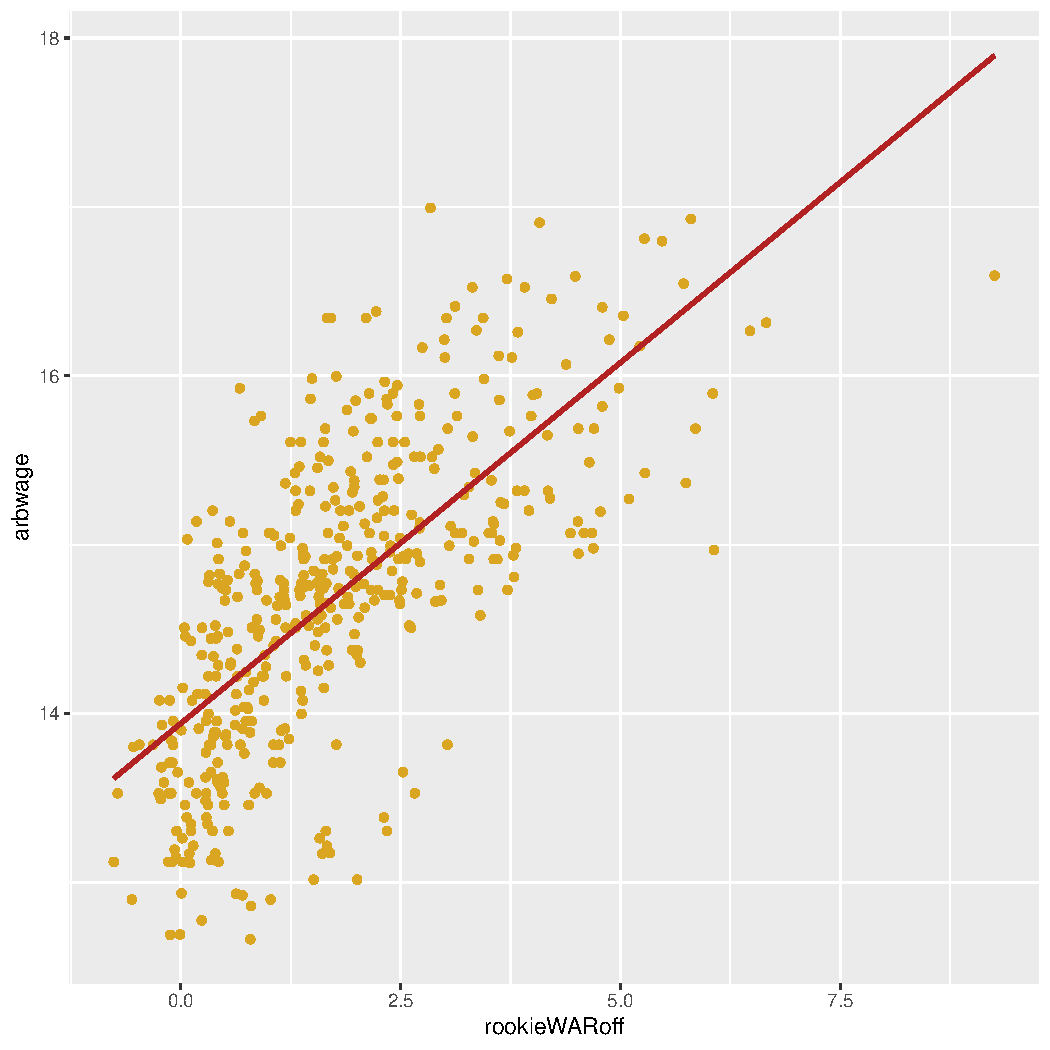
\includepdf[pages=-]{ggplot.pdf}



\end{document}
